%%%% This CV has been greatly influence by
%%%% the extended fancy cv from Carmine Benedetto.
%%%% I thank him for the excellent work. Unfortunately 
%%%% it wouldn't compile on my machine. So I worked it out myself.

\documentclass{article} 
\usepackage[ngerman]{babel}% deutsche Trennregeln
\usepackage{microtype}% verbesserter Randausgleich
\usepackage[utf8]{inputenc}
\usepackage{graphicx}
\usepackage{color}
\usepackage{xcolor}
\usepackage{textcomp}
\usepackage[export]{adjustbox}
\usepackage[obeyspaces]{url} 
\usepackage[left=0.5cm,top=0.25cm,right=0.5cm,bottom=0.5cm,nohead,nofoot]{geometry}

\usepackage{fontawesome}
%https://www.wolframalpha.com/input/?i=seismic+magnitude
\usepackage{svg}

\makeatletter
\setlength{\@fptop}{40pt}
\makeatother

\usepackage{pdfcomment}
% Fix incorrect display of tooltips (http://tex.stackexchange.com/a/74340/3323)
\makeatletter
\renewcommand{\pc@annot@tooltip}%
{%
  /TU (\pc@pdfenc@contents)\space%
  /T (tooltip \thezref@unique)\space%
  /C [0 0 0]\space%
  /FT/Btn\space%
  /Ff 65536\space%
  /H/N\space%
}%

  
\definecolor{white}{RGB}{255,255,255}
\definecolor{anti-flashwhite}{rgb}{0.95, 0.95, 0.96}

\definecolor{darkgray}{HTML}{333333}
\definecolor{gray}{HTML}{4D4D4D}
\definecolor{lightgray}{HTML}{999999}

\definecolor{green}{HTML}{C2E15F}
\definecolor{orange}{HTML}{FDA333}
\definecolor{purple}{HTML}{D3A4F9}
\definecolor{red}{HTML}{FB4485}
\definecolor{blue}{HTML}{6CE0F1}
\definecolor{pblue}{HTML}{0395DE}

\usepackage[framemethod=tikz]{mdframed}
\usepackage{tikz}
\newcommand*{\ClipSep}{0.4cm}%


\usepackage{hyperref}
\hypersetup{
    pdftitle={},
    pdfauthor={},
    pdfsubject={},
    pdfkeywords={},
    colorlinks=false,       % no lik border color
   allbordercolors=white    % white border color for all
}
 
\pagestyle{empty}

\begin{document}
\begin{mdframed}[backgroundcolor=anti-flashwhite]
	\begin{minipage}[t]{0.4\textwidth}
	{\fontsize{30pt}{62pt}\color{gray} \selectfont {Silvio}{\textbf{Schwarz}}}\\
    {\fontsize{14pt}{24pt}\color{pblue} \selectfont Geophysicist \color{lightgray} (B.Sc.)}\\\\
    \textbf{\underline{Philosophy}}:
    \begin{itemize}
    \item open-source, replicable, cross-disciplinary
    \item failure is part of progress
    \item reliability beats sophistication
    \end{itemize}
	\end{minipage}
	\hfill
	\vrule
	\hfill
	\begin{minipage}[t]{0.2\textwidth}
	\vspace{0cm}
	\begin{tikzpicture}
\node [inner sep=0pt] at (0,0) {
\includegraphics[trim=0cm 12cm 0cm 0cm, clip,scale = 0.1]{../img/ich2.jpg}};
\draw [anti-flashwhite, rounded corners=\ClipSep, line width=\ClipSep] 
    (current bounding box.north west) -- 
    (current bounding box.north east) --
    (current bounding box.south east) --
    (current bounding box.south west) -- cycle
    ;
\end{tikzpicture}
	\end{minipage}
	\hfill
	\begin{minipage}[t]{0.25\textwidth}
	\vspace{0.25cm}
	{\color{pblue}Address}\\
	Zeppelinstraße 162, 3.2\\
	14471 Potsdam. Germany
	
	\vspace{0.15cm}
	{\color{pblue}Telephone}\\
	01746507598
	
	\vspace{0.15cm}
	{\color{pblue}Email}\\
	\href{mailto:silvio\_ schwarz@web.de}{silvio{\_}schwarz@web.de}
	
	\vspace{0.15cm}
	{\color{pblue}Web}
	
	\vspace{0.15cm}
	{\Large \href{https://www.silvioschwarz.com}{\faHome} \hfill
	 \href{https://github.com/silvioschwarz}{\faGithub}  \hfill 
	 \href{silvioschwarz.}{\faSkype} \hfill 
	 \href{https://www.linkedin.com/in/silvioschwarz/}{\faLinkedin} \hfill 
	 \href{https://twitter.com/slvschwrz}{\faTwitter} \hfill  
	 \href{www.kaggle.com/amethodtomadness/}{
\includegraphics{../img/kaggle.png}}}
	\end{minipage}
\end{mdframed}
\vfill
\begin{minipage}[t]{0.27\textwidth}
	\centering
	\section*{\hfill\fontsize{18pt}{24pt}\selectfont\color{pblue}Global Experience}
	\vspace{-2mm}
	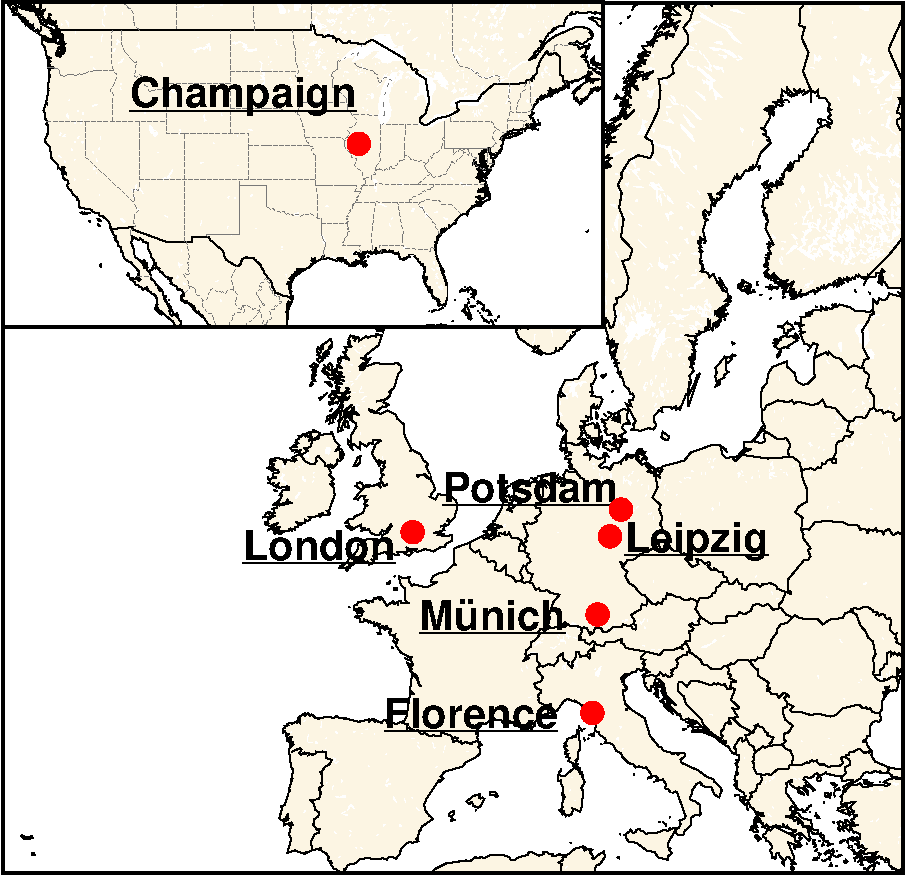
\includegraphics[trim=0.2cm 0.2cm 0.2cm 0.2cm, clip,scale=0.3, frame]{../img/globalEXPENG.pdf}
	\vspace{2mm}
	\hrule
	\vspace{-3mm}
	\section*{\fontsize{18pt}{24pt}\selectfont \color{pblue} OS Preference}
	\vspace{-2mm}
	\begin{itemize}
	\centering
	\item[\textbf{\LARGE \faLinux}]
\includegraphics[trim=0.2cm 0.2cm 0.1cm 0.1cm,clip,scale=0.7]{../img/5stars.png}\vspace{-2mm}
	\item[\textbf{\LARGE \faWindows}]
\includegraphics[trim=0.2cm 0.2cm 0.1cm 0.1cm,clip,scale=0.7]{../img/4stars.png}\vspace{-2mm}
    \item[\textbf{\LARGE \faApple}]
\includegraphics[trim=0.2cm 0.2cm 0.1cm 0.1cm,clip,scale=0.7]{../img/1stars.png}
    \end{itemize}
	\hrule
	\vspace{-2mm}
    \section*{\fontsize{18pt}{24pt}\selectfont \color{pblue} Programming}
	\vspace{-2mm}
	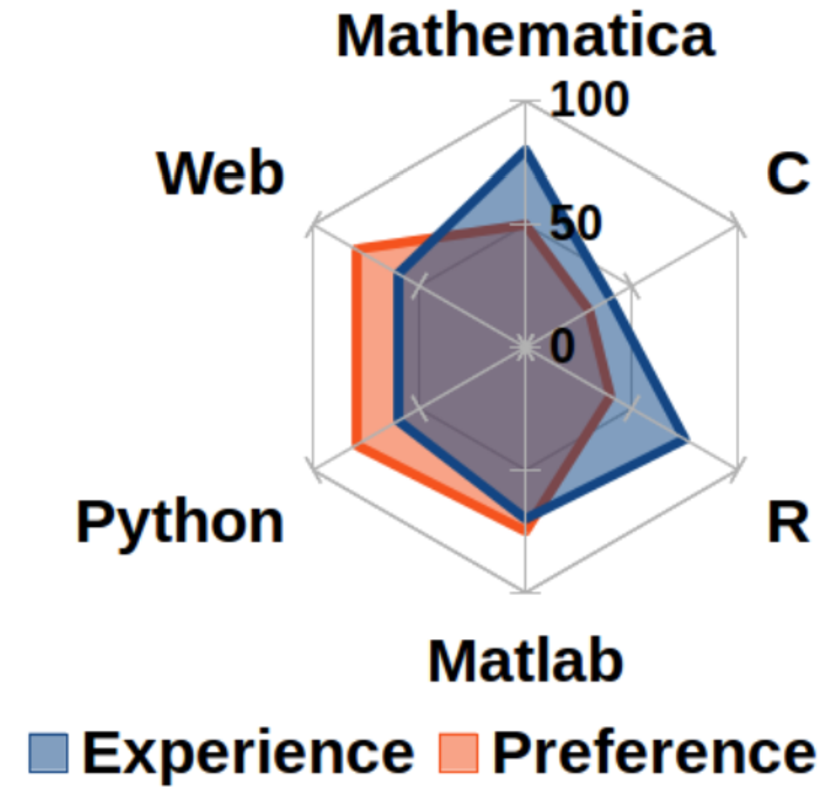
\includegraphics[trim=0.5cm 0.2cm 0.3cm 0.2cm,clip,scale=0.32]{../img/programming.pdf}
	\vspace{2mm}
	\hrule
	\vspace{-2mm}
	\section*{\fontsize{18pt}{24pt}\selectfont \color{pblue} Languages}
	\vspace{-2mm}
	\begin{itemize}
	\centering
	\item[\textbf{\large German}] 
\includegraphics[trim=0.2cm 0.2cm 0.1cm 0.1cm,clip,scale=0.7]{../img/5stars.png}\vspace{-2mm}
	\item[\textbf{\large English}]  
\includegraphics[trim=0.2cm 0.2cm 0.1cm 0.1cm,clip,scale=0.7]{../img/4stars.png}\vspace{-2mm}
    \item[\textbf{\large Italian}] 
\includegraphics[trim=0.2cm 0.2cm 0.1cm 0.1cm,clip,scale=0.7]{../img/3stars.png}\vspace{-2mm}
    \item[\textbf{\large French}]  
\includegraphics[trim=0.2cm 0.2cm 0.1cm 0.1cm,clip,scale=0.7]{../img/2stars.png}
    \end{itemize}
	\hrule
	\vspace{-2mm}
	 \section*{\fontsize{18pt}{24pt}\selectfont \color{pblue} Interests}
	\vspace{-2mm}
	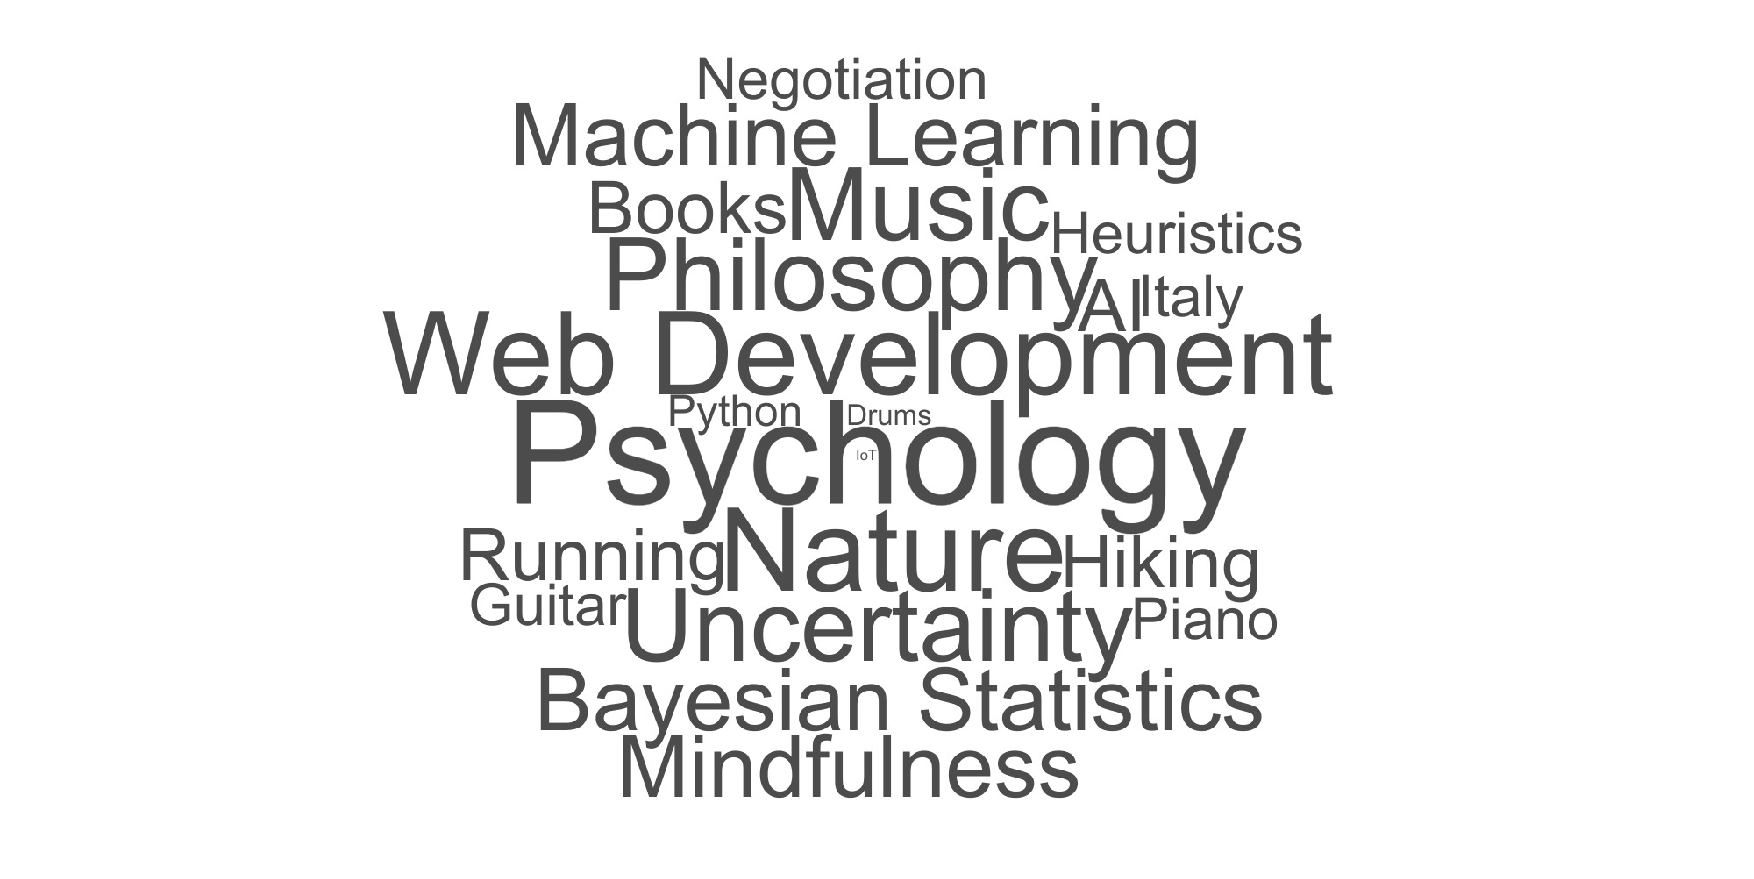
\includegraphics[trim=6cm 1cm 6cm 1cm, clip,scale=0.3]{../img/wordcloud2.pdf}
\end{minipage}
\hfill
\vrule
\hfill
\begin{minipage}[t]{0.7\textwidth}
		\section*{\fontsize{18pt}{24pt}\selectfont \color{pblue} Education}
		
		\begin{minipage}[t]{0.38\textwidth}
	\textbf{\large \color{pblue}\faHourglassHalf\hspace{1mm}Master of Science}\\
	\textbf{\underline{Earth Sciences}}\\
	\textbf{Geophysics,\\ Machine Learning}\\\\
	\begin{minipage}[t]{0.52\textwidth}
	\textbf{\underline{Thesis 1}}:\\
	\textbf{\underline{cancelled}}\footnote{due to illness}\\
	\href{https://github.com/silvioschwarz/master-thesis}{Forecasting Macroseismic Intensities:\\Sensitivity Study of a Bayesian\\ Approach}
	\end{minipage}
	\hfill
	\begin{minipage}[t]{0.45\textwidth}
	\textbf{\underline{Thesis 2}}:\\
	\href{https://github.com/silvioschwarz/master-thesis}{Classification of eruptive tremor sources during the 2014/15\\ Holuhraun eruption, Iceland}
	\end{minipage}
	\\\\\\\
		10/2011 - present\\
	\href{https://www.uni-potsdam.de/}{\color{pblue}Universität Potsdam}
		\end{minipage}		
		\hfill
		\begin{minipage}[t]{0.33\textwidth}
	\textbf{\href{https://www.dropbox.com/s/297g1chiby8mrd3/Bachelor-Certificate.pdf?dl=0}{\large \color{pblue}\faGraduationCap\hspace{1mm}Bachelor of Science}}\\
	\textbf{\underline{Earth Sciences}}\\
	\textbf{Geology, Math, Physics,\\ Chemistry}\\\\
	\textbf{\underline{Thesis}}:\\
	\href{https://www.dropbox.com/s/3kngo4hpb0c47ww/Bachelorarbeit.pdf?dl=0}{\pdftooltip{Simulation von Bodenbewegungsszenarien von Starkbeben (German)}{engl.: Simulating Ground Motion Scenarios of strong Earthquakes}}\\\\\\
	Simulating Ground Motion Scenarios of strong Earthquakes\\\\\\
	{10/2008 - 09/2011}\\
\href{https://www.uni-potsdam.de/}{\color{pblue}Universität Potsdam}\\\\
		\end{minipage}
		\hfill
		\begin{minipage}[t]{0.25\textwidth}
	\textbf{\large \href{https://www.dropbox.com/s/nsgmvy7o64xb9si/Abiturzeugnis.pdf?dl=0}{\color{pblue}\faGraduationCap\hspace{1mm}Abitur}}\\
	\textbf{\underline{Exams:}}\\
	\textbf{Maths, Geography, English, Philosophy}\\\\
	\textbf{\underline{Thesis}}:\\
	 \pdftooltip{Naturkatastrophen und ihr Einfluss auf das Leben im 21.Jahrhundert\\ (German)}{engl.: Natural Disasters and their Impact on Life in the $21^{st}$ century}\\\\
	  Natural Disasters and their Impact on Life in the  $21^{st}$ century\\\\
	 08/2000 - 05/2008\\
	 \href{https://www.klosterschule.de/}{\color{pblue}Klosterschule Roßleben}
		\end{minipage}
		\vspace{-5mm}
		\hrule
		\vspace{-1mm}
		\section*{\fontsize{18pt}{24pt}\selectfont \color{pblue} Work Experience}
		
		\begin{minipage}[t]{0.52\textwidth}
		%\vspace{-60mm}
		\begin{minipage}[t]{0.25\textwidth}
		\centering
		11/2017\\ -\\ 03/2018\\(5 months)
		\end{minipage}
		\hfill
		\begin{minipage}[t]{0.75\textwidth}
		\textbf{Student Trainee}\\ \href{https://assecor.de/}{\color{pblue}DB Dialog}\\
	    Customer Support in\\ passenger rights
		\end{minipage}
		
		\vspace{0.2cm}

		
		\begin{minipage}[t]{0.25\textwidth}
		\centering
		08/2014\\ -\\ 06/2015\\(11 months)
		\end{minipage}
		\hfill
		\begin{minipage}[t]{0.75\textwidth}
		\textbf{Student Trainee}\\
		\href{https://assecor.de/}{\color{pblue}Assecor GmbH}\\
	    GIS Documentation of the \\power grid Berlin, Germany for \\Vattenfall Europe Sales GmbH
		\end{minipage}
	
		\vspace{0.2cm}
			
		\begin{minipage}[t]{0.25\textwidth}
		\centering
		11/2013\\ -\\ 03/2014 \\(5 months)
		\end{minipage}
		\hfill
		\begin{minipage}[t]{0.75\textwidth}
		\textbf{Student Trainee}\\
		\href{https://assecor.de/}{\color{pblue}Assecor GmbH}\\
	     Migration of the IT Infrastructure for BIOTRONIK SE \& Co. KG
		\end{minipage}
		
		\vspace{0.3cm}
				
		\subsection*{\fontsize{18pt}{24pt}\selectfont \color{pblue} Projects}
		\begin{itemize}
		\item \textbf{\color{pblue}\underline{\color{pblue} \large TerremotoPi}} \href{https://github.com/silvioschwarz/TerremotoPi}{\Large \faGithub} \\
		Live stream ground motion, powered by RaspberryPi\textsuperscript{\textregistered}
		\item  \textbf{\color{pblue}\underline{\color{pblue} \large EQ:S2S}} \href{https://github.com/silvioschwarz/Earthquake-Distances}{\Large \faGithub}\\
			Source-to-Site distances for Earthquakes
		\item  \textbf{\color{pblue}\underline{\color{pblue}\large HackHPI'19: TerrorXAfrica}} \href{https://github.com/silvioschwarz/TerrorXAfrica}{\Large \faGithub}\\
		(read: Terror across Africa)\\
			Fighting Terrorism across Africa through the means of data science!
		\end{itemize}
		\end{minipage}	
		\hfill
		\vrule	
		\hfill
		\begin{minipage}[t]{0.45\textwidth}

\begin{minipage}[t]{0.25\textwidth}
		\centering
		05/2019\\ -\\ 11/2019 \\(6 months)
		\end{minipage}
		\hfill
		\begin{minipage}[t]{0.75\textwidth}
		\textbf{Student Researcher}\\
		\href{https://www.uni-potsdam.de/}{\color{pblue}Universität Potsdam}\\
	    Classification of eruptive tremor sources in Iceland\\
	      \textbf{\underline{Supervision}:}\\
	     \href{http://www.geo.uni-potsdam.de/mitarbeiterdetails/show/717/Eva_Eibl.html}{\color{pblue}Prof. Eva Eibl}
		\end{minipage}
		\vspace{0.3cm}
		
		
		%		\begin{minipage}[t]{0.3\textwidth}
%		12/2017 - 03/2018\\ (4 Monate)
%		\end{minipage}
%		\hfill
%		\begin{minipage}[t]{0.7\textwidth}
%		\textbf{studentischer Assistent}\hfill \href{https://gfz-potsdam.de/}{\color{pblue}GFZ Potsdam}\\
%	    Sektion 2.4: Seismologie\\ automatisierte Qualitätskontrolle seismischer Stationen im AlpArray Netzwerk
%		\end{minipage}\vspace{0.5cm}
		
		\begin{minipage}[t]{0.25\textwidth}
		\centering
		09/2012\\ -\\ 11/2012 \\(3 months)
		\end{minipage}		
		\hfill
		\begin{minipage}[t]{0.75\textwidth}
		\textbf{Master Internship}\\
		\href{https:///www.wolframalpha.com/}{\color{pblue}Wolfram$\mid$Alpha, IL, USA}\\
	   Development of geophysical content for Wolfram$~\mid~$Alpha\\
	    \href{https://m.wolframalpha.com/input/?i=moment+magnitude}{\color{pblue}Example}\\
	     \textbf{\underline{Supervision}:}\\
	     \href{mailto:bjornz@wolfram.com }{\color{pblue} Dr. Björn Zimmermann} \\ \href{mailto:mtrott@wolfram.com }{\color{pblue} Dr. Michael Trott} 
		\end{minipage}
		\vspace{0.3cm}
		
	\begin{minipage}[t]{0.25\textwidth}
		\centering
		06/2011\\ -\\ 08/2012 \\(1 year \\3 months)
		\end{minipage}
		\hfill
		\begin{minipage}[t]{0.75\textwidth}
		\textbf{Student Researcher}\\
		\href{https://www.uni-potsdam.de/}{\color{pblue}Universität Potsdam}\\
	    SSHAC LEVEL 3 PSHA\\ model building and consulting\\
	      \textbf{\underline{Supervision}:}\\
	     \href{http://www.geo.uni-potsdam.de/mitarbeiterdetails/show/96/Frank_Scherbaum.html/}{\color{pblue}Prof. Frank Scherbaum}\\
	    1 week Imperial College London: \href{https://www.imperial.ac.uk/people/j.bommer}{\color{pblue}Prof. Julian J. Bommer}
		\end{minipage}
		
		\vspace{0.3cm}
		
		
		\begin{minipage}[t]{0.25\textwidth}
		\centering
		03/2011\\ - \\ 04/2011\\(1 month)
		\end{minipage}		
		\hfill
		\begin{minipage}[t]{0.75\textwidth}
		\textbf{Bachelor Internship}\\
		\href{http://geologie.physgeo.uni-leipzig.de}{\color{pblue}Universität Leipzig}\\
	    Seismological Network of Saxony\\ 
	     \textbf{\underline{Supervision}}: \\
	     \href{mailto:sfunke@rz.uni-leipzig.de}{Dipl. Geophys. S. Funke}
		\end{minipage}
		
%		\begin{minipage}[t]{0.25\textwidth}
%		03/2010 - 05/2010 \\ (3 months)
%		\end{minipage}
%		\hfill
%		\begin{minipage}[t]{0.75\textwidth}
%		\textbf{studentischer Assistent}\\
%		\href{https://www.uni-potsdam.de/}{\color{pblue}Universität Potsdam}\\
%	    Quality control of algorithms used in the scope of seismic hazard analysis\\
%	    Arbeitsgruppe \href{http://www.geo.uni-potsdam.de/mitarbeiterdetails/show/96/Frank_Scherbaum.html}{\color{pblue}Prof. Frank Scherbaum}\	    
%		\end{minipage}
		\end{minipage}		
\end{minipage}
\end{document}